\documentclass[11pt,a4paper]{article}

\usepackage[margin=2.4cm]{geometry}
\usepackage[T1]{fontenc}
\usepackage{mathptmx}
\usepackage{microtype}
\usepackage[table]{xcolor}
\usepackage{booktabs}
\usepackage{longtable}
\usepackage{tabularx}
\usepackage{array}
\usepackage{enumitem}
\usepackage{tikz}
\usetikzlibrary{positioning,arrows.meta,shapes.geometric,fit,backgrounds}
\usepackage{fancyhdr}
\usepackage{titlesec}
\usepackage[hidelinks]{hyperref}

\definecolor{jsblue}{HTML}{000000}
\definecolor{jsnavy}{HTML}{000000}
\definecolor{jspale}{HTML}{F2F2F2}
\definecolor{jsgrey}{HTML}{000000}

\titleformat{\section}{\Large\bfseries\color{jsnavy}}{\thesection}{0.6em}{}
\titleformat{\subsection}{\large\bfseries\color{jsblue}}{\thesubsection}{0.6em}{}
\setlist{itemsep=2pt,topsep=4pt}
\setlength{\parindent}{0pt}
\setlength{\parskip}{6pt}
\renewcommand{\arraystretch}{1.3}
\usepackage{setspace}
\setstretch{1.08}

\pagestyle{fancy}
\fancyhf{}
\lhead{\small\color{jsgrey}JobShield -- Technical Architecture}
\rhead{\small\color{jsgrey}Team Nikolaos}
\cfoot{\small\thepage}
\fancypagestyle{plain}{\fancyhf{}\cfoot{\small\thepage}\renewcommand{\headrulewidth}{0pt}}
\renewcommand{\headrulewidth}{0.3pt}

\newcommand{\tbl}[1]{\textbf{#1}}
\newcommand{\code}[1]{\texttt{\small #1}}

\begin{document}

%-------------------------------------------------------------
% Cover page
%-------------------------------------------------------------
\begin{titlepage}
\thispagestyle{empty}
\centering
\vspace*{2.2cm}
{\large\textsc{NEMISA Digital Innovation Discothon 2026}}\\[0.5cm]
\rule{\textwidth}{0.8pt}\\[1.2cm]
{\fontsize{34}{40}\selectfont\bfseries JobShield}\\[0.5cm]
{\Large A recruitment trust and verification layer for South Africa}\\[1.4cm]
{\fontsize{20}{24}\selectfont\bfseries Technical Architecture Documentation}\\[1.2cm]
\rule{\textwidth}{0.8pt}\\[2.0cm]
{\large\textbf{Team Nikolaos}}\\[0.5cm]
{\large Amar Mustafa\\[2pt] Mintesinot Necha\\[2pt] Keamogetse Maremela}\\[2.2cm]
{\normalsize Challenge: Youth Employment and Digital Entrepreneurship\\[2pt]
Supporting challenge: Cybersecurity, Online Safety and Digital Well-being}\\[1.2cm]
{\normalsize 15 November 2026\\[2pt] Version 1.0}
\vfill
{\small Submitted through the Sonke platform}
\end{titlepage}

%-------------------------------------------------------------
% Table of contents
%-------------------------------------------------------------
\pagenumbering{roman}
\setcounter{page}{2}
\setcounter{tocdepth}{2}
\renewcommand{\contentsname}{Table of Contents}
\tableofcontents
\clearpage

%-------------------------------------------------------------
% Body
%-------------------------------------------------------------
\pagenumbering{arabic}
\setcounter{page}{1}

%-------------------------------------------------------------
\section{Purpose and scope}
%-------------------------------------------------------------
\noindent\fbox{\parbox{0.96\textwidth}{\small\textbf{Summary.} JobShield is a recruitment trust layer. A job seeker forwards a job message or scans a QR code and, within about 30 seconds, gets a plain-language rating (Verified, Unverified or High risk) with the evidence behind it. We promise evidence-backed verification and risk assessment, never a guarantee that a job is genuine.}}

\medskip
This document describes how JobShield is built: its parts, how they talk to each other, what data it keeps, how it stays secure and how it can grow. It supports our Lean Business Canvas, Secure System Development Lifecycle (SSDLC) answers and pitch deck.

\textbf{The problem.} Unemployment among South Africans aged 15 to 34 was 47.4\% in the second quarter of 2026 \cite{qlfs}. Impersonation fraud victims rose by 54\% in 2024 compared with 2023 \cite{safps}, and fake job offers are the most common lure used by human traffickers in South Africa \cite{nfn}.

\textbf{Challenge addressed.} NEMISA's \emph{Youth Employment and Digital Entrepreneurship} challenge asks for digital solutions that help young people access employment opportunities. Young people can only use opportunities they can trust, so JobShield also answers the \emph{Cybersecurity, Online Safety and Digital Well-being} challenge on scams and fraud.

\textbf{What this document is not.} It is a design for a pilot, not a report on a finished product. Where something is planned or simulated, we say so (see Section~\ref{sec:assumptions}). All targets are goals, not results.

\subsection{Design goals}
\begin{itemize}
  \item \textbf{Trustworthy by evidence:} every rating shows what was checked, against which source, and on what date.
  \item \textbf{Fail safe:} if a source is down, the answer is ``could not verify'', never ``verified''.
  \item \textbf{Privacy first:} collect the minimum, keep no ID copies by default, store scam identifiers only as keyed hashes.
  \item \textbf{Low-data and WhatsApp first:} short text answers and small web pages, with no app download needed.
  \item \textbf{Explainable:} clear rules decide; machine learning only supports them; AI text only explains.
  \item \textbf{Free for job seekers:} the Employment Services Act bans fees for work seekers \cite{esa}, so employers and institutions pay.
\end{itemize}

\subsection{Team and responsibilities}
\begin{center}
\begin{tabularx}{\textwidth}{@{}>{\raggedright\arraybackslash}p{3.1cm}>{\raggedright\arraybackslash}X>{\raggedright\arraybackslash}X@{}}
\toprule
\tbl{Member} & \tbl{Experience} & \tbl{Owns in this design}\\
\midrule
Amar Mustafa & Has built software for clients. Marketing experience with Google Ads, Meta Ads and TikTok. & Web app, WhatsApp channel, API and employer portal; launch and awareness.\\
Mintesinot Necha & Experience in business requirements and discussing needs with clients. & Backend infrastructure, deployment, signing service, requirements and project overview.\\
Keamogetse Maremela & Has worked with data at UJ. Quantitative and finance experience. & Risk engine, text similarity, SCAMTRACE analysis, AI explanations and the numbers behind the business model.\\
\bottomrule
\end{tabularx}
\end{center}
All three of us work together on research, design decisions, testing and the pitch.

%-------------------------------------------------------------
\section{Architecture at a glance}
%-------------------------------------------------------------
JobShield is a small set of services behind one secure gateway. People reach it through WhatsApp, a web app or a QR scan. The platform checks trusted sources and returns a signed or explained answer.

\begin{figure}[ht]
\centering
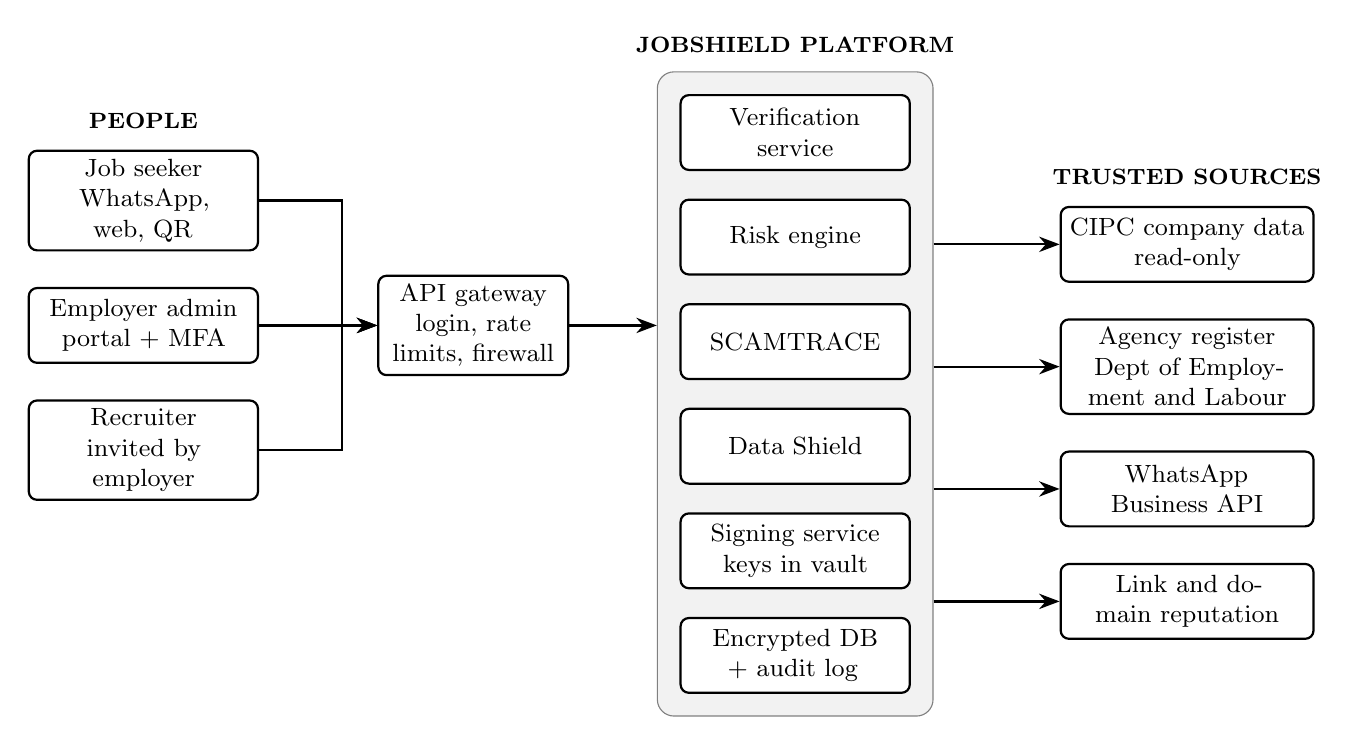
\begin{tikzpicture}[
  font=\small,
  box/.style={draw=jsblue, thick, rounded corners=3pt, fill=white, align=center, minimum height=0.95cm, text width=2.7cm, inner sep=3pt},
  src/.style={draw=jsnavy, thick, rounded corners=3pt, fill=white, align=center, minimum height=0.95cm, text width=3.0cm, inner sep=3pt},
  grp/.style={draw=black!50, fill=jspale, rounded corners=6pt, inner sep=8pt},
  arr/.style={-{Stealth[length=2.6mm]}, thick, color=jsblue},
  lbl/.style={font=\footnotesize\bfseries, color=jsblue}
]
% people
\node[box] (seeker) {Job seeker\\ WhatsApp, web, QR};
\node[box, below=0.45cm of seeker] (employer) {Employer admin\\ portal + MFA};
\node[box, below=0.45cm of employer] (recruiter) {Recruiter\\ invited by employer};
\node[lbl, above=0.15cm of seeker] {PEOPLE};

% gateway
\node[box, right=1.5cm of employer, text width=2.2cm] (gw) {API gateway\\ login, rate limits, firewall};

% services
\node[box, right=1.4cm of gw, yshift=2.45cm] (ver) {Verification\\ service};
\node[box, below=0.35cm of ver] (risk) {Risk engine};
\node[box, below=0.35cm of risk] (scam) {SCAMTRACE};
\node[box, below=0.35cm of scam] (shield) {Data Shield};
\node[box, below=0.35cm of shield] (sign) {Signing service\\ keys in vault};
\node[box, below=0.35cm of sign] (db) {Encrypted DB\\ + audit log};
\begin{scope}[on background layer]
  \node[grp, fit=(ver)(risk)(scam)(shield)(sign)(db)] (plat) {};
\end{scope}
\node[lbl, above=0.12cm of plat.north] {JOBSHIELD PLATFORM};

% sources
\node[src, right=1.6cm of plat.east, yshift=1.9cm] (cipc) {CIPC company data\\ read-only};
\node[src, below=0.45cm of cipc] (del) {Agency register\\ Dept of Employment and Labour};
\node[src, below=0.45cm of del] (wa) {WhatsApp Business API};
\node[src, below=0.45cm of wa] (link) {Link and domain reputation};
\node[lbl, above=0.15cm of cipc] {TRUSTED SOURCES};

\draw[arr] (seeker.east) -| ([xshift=-0.45cm]gw.west) -- (gw.west);
\draw[arr] (employer.east) -- (gw.west);
\draw[arr] (recruiter.east) -| ([xshift=-0.45cm]gw.west) -- (gw.west);
\draw[arr] (gw.east) -- (plat.west |- gw.east);
\draw[arr] (plat.east |- cipc.west) -- (cipc.west);
\draw[arr] (plat.east |- del.west) -- (del.west);
\draw[arr] (plat.east |- wa.west) -- (wa.west);
\draw[arr] (plat.east |- link.west) -- (link.west);
\end{tikzpicture}
\caption{JobShield components. Government checks use approved APIs or imported registers; the prototype uses a labelled demo dataset.}
\label{fig:arch}
\end{figure}

\subsection{Component responsibilities}
\begin{center}
\small
\begin{tabularx}{\textwidth}{@{}>{\raggedright\arraybackslash}p{3.0cm}>{\raggedright\arraybackslash}X>{\raggedright\arraybackslash}p{4.3cm}@{}}
\toprule
\tbl{Component} & \tbl{What it does} & \tbl{Proposed technology}\\
\midrule
Channels & WhatsApp bot, installable web app, QR scan, employer portal & WhatsApp Business API, React web app\\
API gateway & Authentication, rate limits, web application firewall, request logging & Managed gateway and firewall\\
Verification service & Checks employer, recruiter and vacancy records and passport signatures & Python (FastAPI)\\
Risk engine & Rules first, then a light ML model and text similarity, then a plain-language reason & Python, scikit-learn\\
SCAMTRACE & Links reports that share a phone number, bank account, website or message template & PostgreSQL graph tables first; a graph database later\\
Data Shield & Records consent and tells the user what is safe to share now & Same API, separate module\\
Signing service & Issues and revokes Verified Vacancy Passports & Ed25519 signatures, keys in a managed vault\\
Data stores & Encrypted database and append-only audit log & PostgreSQL, encrypted at rest\\
Outside sources & CIPC company API, agency registration records, link reputation & Read-only calls over TLS\\
\bottomrule
\end{tabularx}
\end{center}

%-------------------------------------------------------------
\section{Key flows}
%-------------------------------------------------------------
\subsection{Check-a-Job (job seeker)}
\begin{enumerate}
  \item The job seeker forwards a message, link or phone number to the JobShield WhatsApp number, or scans a passport QR code.
  \item The gateway authenticates the request, applies rate limits and passes it on.
  \item \textbf{If it is a passport QR:} the verification service checks the signature, the expiry date and the revocation list, then shows the employer, recruiter and vacancy.
  \item \textbf{If it is a message:} the risk engine extracts signals (payment request, links, sender number, wording), checks SCAMTRACE and the official sources, and produces a rating.
  \item The answer returns in plain language with the evidence and the date of each check.
  \item If the user reports a scam, SCAMTRACE stores keyed hashes of the identifiers and links them to earlier reports.
\end{enumerate}

\subsection{Issue a Verified Vacancy Passport (employer)}
\begin{enumerate}
  \item The employer registers with its company name and registration number.
  \item JobShield matches the company record and confirms the request on an independent company channel (for example, a listed company email or phone).
  \item The employer admin invites a recruiter and chooses which vacancies that recruiter may advertise.
  \item The admin approves the vacancy, the recruiter and the official application link.
  \item The signing service issues a signed passport with an expiry date. The employer can revoke it at any time.
\end{enumerate}

\subsection{Three checks behind every passport}
\begin{center}
\begin{tabularx}{\textwidth}{@{}lXX@{}}
\toprule
\tbl{Check} & \tbl{Question} & \tbl{Evidence used}\\
\midrule
1. Employer identity & Is the employer a real, active company? & CIPC company record, independent confirmation, manual review for hard cases\\
2. Recruiter authority & Is this person or agency allowed to recruit for that employer? & Employer-signed invitation, agency registration record\\
3. Vacancy approval & Did the employer approve this exact vacancy and apply link? & Approval by the employer admin, signed and time-limited\\
\bottomrule
\end{tabularx}
\end{center}

%-------------------------------------------------------------
\section{Interfaces}
%-------------------------------------------------------------
The platform exposes one versioned REST API. The WhatsApp bot and the web app are clients of the same API.

\begin{center}
\small
\begin{tabularx}{\textwidth}{@{}>{\raggedright\arraybackslash}p{5.1cm}>{\raggedright\arraybackslash}p{2.3cm}X@{}}
\toprule
\tbl{Endpoint} & \tbl{Caller} & \tbl{Purpose}\\
\midrule
\code{POST /v1/check} & Job seeker & Submit a message, link or number and get a rating with reasons\\
\code{GET /v1/passport/\{id\}} & Anyone & Verify a passport: signature, expiry, revocation, linked records\\
\code{POST /v1/report} & Job seeker & Report a scam; identifiers are stored only as keyed hashes\\
\code{POST /v1/employer/vacancies} & Employer admin & Create or approve a vacancy and application link\\
\code{POST /v1/employer/recruiters} & Employer admin & Invite a recruiter and set allowed vacancies\\
\code{POST /v1/passport/\{id\}/revoke} & Employer admin & Revoke a passport immediately\\
\bottomrule
\end{tabularx}
\end{center}

\textbf{Passport contents.} A passport holds the vacancy ID, employer ID, recruiter ID, issue and expiry dates, a random nonce and an Ed25519 signature \cite{rfc8032}. The QR code carries only the passport link, so the data lives on our side and revocation takes effect immediately.

%-------------------------------------------------------------
\section{Data model}
%-------------------------------------------------------------
\begin{center}
\small
\begin{tabularx}{\textwidth}{@{}>{\raggedright\arraybackslash}p{2.4cm}>{\raggedright\arraybackslash}X>{\raggedright\arraybackslash}p{3.2cm}@{}}
\toprule
\tbl{Record} & \tbl{Key fields} & \tbl{Personal data?}\\
\midrule
Employer & Name, registration number, verified date, status & No\\
Recruiter & Name, agency, employer, allowed vacancies, status & Yes, minimal\\
Vacancy & Title, employer, recruiter, apply link, expiry, status & No\\
Passport & Vacancy ID, signature, issue and expiry dates, revoked flag & No\\
Check log & Time, result, reasons (no message text kept by default) & Minimal\\
Scam report & Keyed hash of phone number, account or website, template fingerprint, date & Hashed only\\
\bottomrule
\end{tabularx}
\end{center}

\textbf{Why keyed hashes.} South African phone numbers are a small search space, so a plain hash could be reversed by trying every number. We use an HMAC with a secret key held in the vault, so linked reports can still be matched but the numbers cannot be read back from the database.

\textbf{Applicant Data Shield.} The user is told what is safe to share at each stage: CV first, ID only after a written offer, banking details only after signing. JobShield stores no copies of ID documents by default.

%-------------------------------------------------------------
\section{Risk engine}
%-------------------------------------------------------------
The risk engine turns signals into a rating. It is built so that every rating can be explained to the user.

\begin{enumerate}
  \item \textbf{Transparent rules.} Examples: asks for a payment; asks for ID or bank details before an interview; sender uses a free email address while claiming to be a company; phone number or website appears in SCAMTRACE; link domain is very new; vacancy not found among verified vacancies.
  \item \textbf{Light machine learning.} A small classifier (scikit-learn) and text similarity against known scam templates find new wording the rules miss. It supports the rules and never overrides a hard rule.
  \item \textbf{AI explanations.} A language model only turns the rule hits and evidence into a short, plain-language explanation. It cannot change the rating. Input text is treated as untrusted to reduce prompt-injection risk.
\end{enumerate}

\textbf{Rating logic.} \emph{Verified} only when a valid, unexpired, unrevoked passport matches. \emph{High risk} when a hard rule fires or the combined score passes a threshold. Otherwise \emph{Unverified}. If a source cannot be reached, the answer says \emph{could not verify}.

\textbf{Pilot targets.} At least 90\% of known scam samples flagged and at most 5\% false alarms on our labelled test set. These are goals to test, not results.

%-------------------------------------------------------------
\section{Security architecture}
\label{sec:security}
%-------------------------------------------------------------
Security is part of the design from the start, following our SSDLC: risk assessment, threat modelling, secure coding, security testing and safe release. We build for the Protection of Personal Information Act (POPIA) \cite{popia}, the Employment Services Act \cite{esa} and the Cybercrimes Act \cite{cca}. Our lifecycle follows the NIST Secure Software Development Framework \cite{ssdf}, and we use the OWASP Top~10 and ASVS as checklists \cite{owasp}.

\subsection{Threat model (STRIDE)}
We classify threats with the STRIDE model \cite{stride}: spoofing, tampering, repudiation, information disclosure, denial of service and elevation of privilege.

\begin{center}
\small
\begin{tabularx}{\textwidth}{@{}>{\raggedright\arraybackslash}p{3.0cm}>{\raggedright\arraybackslash}p{2.2cm}>{\raggedright\arraybackslash}X@{}}
\toprule
\tbl{Threat} & \tbl{STRIDE} & \tbl{Control}\\
\midrule
Fake employer signs up & Spoofing & Company record match, independent confirmation, manual review\\
Stolen employer login & Spoofing, Elevation & Multi-factor sign-in, signed approvals, alerts on new devices\\
Forged or copied QR & Tampering & Ed25519 signatures, expiry, instant revocation, link-based verification\\
Leak of applicant data & Information disclosure & Collect the minimum, encrypt at rest and in transit, no ID copies stored\\
False or abusive reports & Tampering, Repudiation & Evidence thresholds, rate limits, audit log, appeal route\\
Flooding the WhatsApp number & Denial of service & Rate limits per number, queueing, cached official data\\
Prompt injection through forwarded text & Tampering & AI only explains, never decides; input treated as untrusted\\
Insider misuse & Elevation, Repudiation & Least privilege, separate signing keys, append-only audit log\\
\bottomrule
\end{tabularx}
\end{center}

\subsection{Controls}
\begin{itemize}
  \item \textbf{In transit and at rest:} TLS everywhere; database and backups encrypted; keys and secrets only in a managed vault.
  \item \textbf{Access:} multi-factor sign-in for employers and staff; role-based access; least privilege between services.
  \item \textbf{Code:} code review, dependency scanning, secrets scanning and static checks in the build pipeline.
  \item \textbf{Testing:} OWASP ZAP scans in the pipeline, unit tests for the rules, and an external penetration test before the pilot goes public (budgeted in our canvas).
  \item \textbf{Privacy:} privacy notice, consent records, data minimisation, retention limits and a deletion route to support POPIA rights.
  \item \textbf{Monitoring:} logs, uptime and error alerts, and an incident plan that includes notifying affected people and the Information Regulator when required.
\end{itemize}

%-------------------------------------------------------------
\section{Deployment, performance and scaling}
%-------------------------------------------------------------
\begin{itemize}
  \item \textbf{Region:} a South African cloud region (for example AWS Cape Town \cite{aws}) so data stays in the country.
  \item \textbf{Environments:} separate test and production, defined as code so they can be rebuilt.
  \item \textbf{Pilot size:} one small deployment (two application servers and one database). Services are stateless, so they can scale sideways when traffic grows.
  \item \textbf{Speed:} slow work (outside-source checks) goes through a queue, official data is cached with its fetch date, and the bot sends a quick acknowledgement first.
  \item \textbf{Design targets:} passport check in under 3 seconds and message check in under 15 seconds for typical requests (targets to test, not measured results).
  \item \textbf{Low data:} short text answers, small pages, no app download.
  \item \textbf{Resilience:} automated backups, tested restores, monitoring and alerts as set out in the SSDLC.
\end{itemize}

%-------------------------------------------------------------
\section{Technology choices}
%-------------------------------------------------------------
\begin{center}
\small
\begin{tabularx}{\textwidth}{@{}>{\raggedright\arraybackslash}p{3.0cm}>{\raggedright\arraybackslash}p{3.6cm}X@{}}
\toprule
\tbl{Layer} & \tbl{Choice} & \tbl{Why}\\
\midrule
Web app & React, installable on a phone & Fast to build, works offline-first for the shell, familiar to the team\\
Backend & Python with FastAPI & Same language as the data and AI work; typed, quick to build and test\\
Database & PostgreSQL & Reliable, encrypted at rest, can model the scam graph before we need a graph database\\
Messaging & WhatsApp Business API \cite{meta} & Where job seekers already are; no app to install\\
Signing & Ed25519 with a managed vault & Small, fast signatures; keys never sit in application code\\
ML & scikit-learn & Light, explainable models that run on a small server\\
Infrastructure & Cloud region in South Africa, infrastructure as code & Data residency and repeatable setups\\
\bottomrule
\end{tabularx}
\end{center}

%-------------------------------------------------------------
\section{Assumptions, limits and what is next}
\label{sec:assumptions}
%-------------------------------------------------------------
\subsection{Honest limits}
\begin{itemize}
  \item CIPC's API needs approval and a paid subscription \cite{cipc}. The prototype uses a labelled demo dataset for company checks.
  \item We could not confirm a public, searchable agency register from the Department of Employment and Labour, so the prototype uses an imported sample and labels it as simulated.
  \item The risk engine is trained and tested on a small labelled set of public scam examples. Pilot targets are goals, not results.
  \item JobShield gives evidence and a risk rating. It never guarantees that a job is genuine.
  \item Our prices, costs and user targets are estimates that we plan to test with interviews and a pilot.
\end{itemize}

\subsection{Build plan}
\begin{center}
\begin{tabularx}{\textwidth}{@{}>{\raggedright\arraybackslash}p{3.0cm}X@{}}
\toprule
\tbl{Stage} & \tbl{What we build or prove}\\
\midrule
Discothon weekend & Clickable prototype of Check-a-Job and the Verified Vacancy Passport on a labelled demo dataset, plus the architecture and SSDLC evidence\\
Months 1 to 3 & Pilot at UJ: WhatsApp bot, passport issuing for about 10 pilot employers, first SCAMTRACE links, penetration test\\
Months 4 to 9 & Grow to TVET colleges, add the employer dashboard and the real CIPC and agency integrations once approved\\
Months 10 to 12 & Harden, scale, add the scam-intelligence API for partners (year 2)\\
\bottomrule
\end{tabularx}
\end{center}

%-------------------------------------------------------------
% References
%-------------------------------------------------------------
\clearpage
\addcontentsline{toc}{section}{References}
\begin{thebibliography}{99}
\setlength{\itemsep}{6pt}
\bibitem{qlfs} Statistics South Africa. \emph{Quarterly Labour Force Survey}, second and third quarters of 2026. Pretoria: Statistics South Africa.
\bibitem{safps} Southern African Fraud Prevention Service (SAFPS). \emph{Annual Fraud Statistics for 2024}, as reported by Daily Investor.
\bibitem{nfn} National Freedom Network. Reporting on job-offer lures used in human trafficking in South Africa, as reported by eNCA.
\bibitem{esa} Republic of South Africa. \emph{Employment Services Act 4 of 2014}. Pretoria: Government Gazette.
\bibitem{popia} Republic of South Africa. \emph{Protection of Personal Information Act 4 of 2013}. Pretoria: Government Gazette.
\bibitem{cca} Republic of South Africa. \emph{Cybercrimes Act 19 of 2020}. Pretoria: Government Gazette.
\bibitem{owasp} OWASP Foundation. \emph{OWASP Top 10} and \emph{OWASP Application Security Verification Standard (ASVS)}. owasp.org.
\bibitem{stride} Hernan, S., Lambert, S., Ostwald, T. and Shostack, A. (2006). Uncover Security Design Flaws Using the STRIDE Approach. \emph{MSDN Magazine}, November 2006.
\bibitem{ssdf} National Institute of Standards and Technology (2022). \emph{Secure Software Development Framework (SSDF) Version 1.1}, NIST Special Publication 800-218.
\bibitem{rfc8032} Josefsson, S. and Liusvaara, I. (2017). \emph{Edwards-Curve Digital Signature Algorithm (EdDSA)}. RFC 8032, Internet Engineering Task Force.
\bibitem{cipc} Companies and Intellectual Property Commission (CIPC). Published API and company disclosure price list. cipc.co.za.
\bibitem{meta} Meta. \emph{WhatsApp Business Platform pricing} for South Africa. developers.facebook.com.
\bibitem{aws} Amazon Web Services. \emph{Africa (Cape Town) region} service pricing. aws.amazon.com.
\end{thebibliography}

\end{document}
